\documentclass[11pt]{article}

\usepackage[margin=1in]{geometry}
\usepackage{amsmath,amssymb,amsthm}
\usepackage{enumitem}
\usepackage{hyperref}
\usepackage{xcolor}
\usepackage{titlesec}
\usepackage{booktabs}
\usepackage{array}
\usepackage{graphicx}
\usepackage[htt]{hyphenat}   % allow \texttt{} to hyphenate at underscores
\usepackage{tikz}
\usetikzlibrary{arrows.meta, positioning, calc}

\hypersetup{
    colorlinks=true,
    linkcolor=blue!50!black,
    citecolor=blue!50!black,
    urlcolor=blue!50!black
}

\newtheorem{theorem}{Theorem}
\newtheorem{proposition}{Proposition}
\newtheorem{corollary}{Corollary}
\theoremstyle{definition}
\newtheorem{definition}{Definition}
\theoremstyle{remark}
\newtheorem{remark}{Remark}

\title{\Large \textbf{Understanding Is Not Observable}\\[4pt]
\large Shared Convention Makes Communication Possible and Its Measurement Impossible}

\author{\textbf{Ashok Pasala} \\[2pt] \small VIT-AP University \\[2pt] \small \texttt{Working Draft v0.1.0}}

\date{July 2026}

\begin{document}

\maketitle

\begin{center}
\colorbox{yellow!20}{\parbox{0.92\textwidth}{\small \textbf{Status:} Working draft. Theorem~\ref{thm:nonid} is complete. Proposition~\ref{prop:gap} is supported by a controlled ground-truth simulation (Section~\ref{sec:empirical}). The interventional protocol of Section~\ref{sec:remedy} has not yet been applied to human--AI or hyperscanning data; those are the paper's principal outstanding obligations.}}
\end{center}

\vspace{6pt}

\begin{abstract}
\noindent
Four fields ask whether one system understands another --- artificial intelligence of its models, neuroscience of interacting brains, comparative cognition of other species, philosophy of other minds --- and all four answer the same way: observe what passes between the systems and infer from it. We show this cannot work, for two independent reasons. First, we prove a non-identifiability result: because any two systems that can communicate must already share prior convention, and shared convention is a common cause of both what is transmitted and how the receiver behaves, there exist dyads with \emph{identical} observational distributions over signals, internal states, and behaviour, one genuinely coupled and one not. No functional of the observational distribution --- mutual information, transfer entropy, neural synchrony, representational similarity, behavioural agreement, or conversational performance --- distinguishes them. The very thing that makes communication possible is what makes it unmeasurable from observation. Second, and independently of confounding, we demonstrate with complete ground truth that coupling measured at the level of \emph{internal states} does not imply coupling at the level of \emph{behaviour}: in a system where the sender encodes its private state into the channel at $R^2 = 0.90$ and a decoder recovers that state from the receiver's hidden layer to a reconstruction error of $0.0017$, the receiver captures at most $12\%$ of what that information is worth, performing at the goal-blind optimum. Removing the channel entirely and handing the receiver the sender's state directly --- infinite bandwidth, zero noise --- changes nothing. We also find that randomising a signal is a materially more sensitive probe than ablating it, and that behavioural sensitivity and functional benefit come apart in turn, so interventional tests must be calibrated against the value of the information rather than against zero. We then characterise what does suffice. Functional coupling is identified by adjustment when the shared convention is observed, by instrumental variation --- for which, we note, ordinary channel noise qualifies, inverting the usual impulse to denoise --- or by direct intervention. Two things notably do not suffice: temporal precedence, so that transfer entropy and Granger causality inherit the full force of the negative result despite being called directional; and observation of the receiver's internal state, which fails the front-door criterion for structural reasons that no gain in recording resolution or interpretability precision can repair. We conclude that functional coupling is an \emph{interventional} quantity sitting one rung above where it is currently measured, and that this, rather than any deep obscurity in the phenomenon, is why debates about machine understanding do not resolve. We derive consequences for AI evaluation, mechanistic interpretability, and hyperscanning, and note that the framework retrodicts the decade-long stagnation of brain-to-brain interface bandwidth.
\end{abstract}

\section{Introduction}

A recurring question appears in several sciences at once, in slightly different dress each time.

Artificial intelligence asks whether a model understands an instruction, and answers with benchmarks, preference ratings, and dialogue. Neuroscience asks whether two brains in interaction are coupled, and answers with inter-brain synchrony and directed information. Comparative cognition asks whether an animal grasps a signal. Developmental psychology asks it of infants. Philosophy asks it in general and calls it the problem of other minds, historically concluding that it is not empirically tractable.

Each field attacks the question with the same instrument: \emph{watch what passes between the two systems, and infer understanding from the pattern}. Score the outputs. Measure the correlation between internal states. Decode one system's content from the other's activity.

This paper argues that the instrument cannot return the answer --- not because measurement is noisy or the systems are complex, but because the quantity of interest is not a function of the data being collected. We give two independent arguments, one theoretical and one empirical, and one remedy.

The theoretical argument (Section~\ref{sec:nonid}) is an identifiability result with an unusual structure. Ordinary confounding is a nuisance that careful design can sometimes remove. Here the confounder cannot be removed, because it is the precondition of the phenomenon. Two systems can only communicate if they already share a convention governing what signals mean. That shared convention is a common cause of what the sender emits and how the receiver behaves. Any observed coherence between them is therefore explicable \emph{either} by the channel doing work \emph{or} by both parties independently instantiating a convention they already held --- and no observational statistic separates these. The prerequisite for communication is the confounder for its measurement.

The empirical argument (Section~\ref{sec:empirical}) is independent and does not rely on confounding at all. In a fully observable artificial system with ground truth over every variable, we exhibit a receiver whose internal state provably contains the sender's private information and whose behaviour provably ignores it. State-level coupling is at ceiling; functional coupling is at floor. Since essentially all neural coupling measures and all interpretability findings are state-level, this is a direct demonstration that such measures do not license behavioural conclusions.

The remedy (Section~\ref{sec:remedy}) follows from the diagnosis. If functional coupling is not identified by observation, it must be identified by intervention: ablate or randomise the channel and measure whether behaviour changes. What survives the removal of a signal is what the signal was doing. Everything else is fluency.

We are not claiming to have solved semantics, and we do not use ``understanding'' in a phenomenal or philosophical sense. Throughout, \emph{functional coupling} names a specific causal quantity: the extent to which one system's signal changes what another system does. Our claim is that this modest, operational quantity --- not consciousness, not meaning in any rich sense --- is already unidentifiable by the methods four fields currently use, and that this is enough to invalidate a substantial body of inference.

\subsection{Contributions}
\begin{enumerate}[leftmargin=*, itemsep=2pt]
    \item A non-identifiability theorem for functional coupling under shared convention (Theorem~\ref{thm:nonid}), with the observation that the confounder is constitutive rather than incidental.
    \item A matching positive result (Theorem~\ref{thm:id}) giving three sufficient conditions for identification, together with two sharp negatives: temporal-precedence measures such as transfer entropy do \emph{not} escape the theorem (Proposition~\ref{prop:time}), and receiver-side measurement does not rescue it via the front-door criterion (Proposition~\ref{prop:frontdoor}).
    \item A ground-truth demonstration that state-level coupling and behaviour-level coupling dissociate completely, including an infinite-bandwidth control (Proposition~\ref{prop:gap}, Section~\ref{sec:empirical}).
    \item An account of why the gap arises --- coupling is a jointly held convention, an attractor of shared history, which cannot be established unilaterally (Section~\ref{sec:why}).
    \item An interventional measurement protocol, and its specialisation to AI evaluation, interpretability, and hyperscanning (Sections~\ref{sec:remedy}--\ref{sec:implications}).
    \item A retrodiction: the framework explains the decade-long flatness of brain-to-brain interface throughput against large hardware gains (Section~\ref{sec:bbi}).
\end{enumerate}

\section{Setup}\label{sec:setup}

Consider a dyad consisting of a sender $A$ and a receiver $B$ exchanging signals over some channel.

\begin{definition}[Dyad]
A dyad is a tuple $\mathcal{D} = (Z_A, M, Z_B, U)$ of random variables, where $Z_A$ is the sender's internal state, $M$ is the signal crossing the channel, $Z_B$ is the receiver's internal state, and $U$ is the receiver's behaviour, together with a causal model specifying how each is generated.
\end{definition}

We are deliberately permissive about what these denote. In hyperscanning, $Z_A, Z_B$ are neural recordings and $M$ is speech, gesture, or gaze. In human--AI interaction, $Z_A$ is the user's intent, $M$ the prompt, $Z_B$ the model's activations, $U$ its output. In multi-agent learning they are agent states and messages. The argument is indifferent to substrate.

One further ingredient is not part of the tuple, precisely because it is generally unobserved: a convention-bearing latent $C$ --- the code, language, or learned protocol the dyad already shares, without which $M$ could not function as a signal at all. Section~\ref{sec:nonid} introduces it formally; it is flagged here because it is the reason the tuple above, exhaustive as it looks, is not enough to determine $\mathcal{F}$.

\begin{definition}[Observational measures]
An \emph{observational} coupling measure is any functional $\Phi$ of the joint distribution $P(Z_A, M, Z_B, U)$ obtained by passive observation of the dyad.
\end{definition}

This class is broad and contains, to our knowledge, every measure currently in use: mutual information $I(Z_A;Z_B)$ and its lagged variants; transfer entropy $\mathrm{TE}_{A\to B}$ \cite{schreiber2000measuring} and Granger causality \cite{granger1969investigating}; directed information \cite{permuter2009directed}; phase-locking and coherence measures in hyperscanning \cite{montague2002hyperscanning, hasson2010brain}; representational similarity and cross-subject decoding; behavioural agreement scores; and performance on conversational benchmarks including the imitation game \cite{turing1950computing}.

\begin{definition}[Functional coupling]\label{def:fc}
The functional coupling of a dyad is the causal dependence of the receiver's behaviour on the signal:
\[
\mathcal{F}(\mathcal{D}) > 0 \quad\Longleftrightarrow\quad \exists\, m, m' : \; P\big(U \mid \mathrm{do}(M{=}m)\big) \;\neq\; P\big(U \mid \mathrm{do}(M{=}m')\big),
\]
where $\mathrm{do}(\cdot)$ is Pearl's intervention operator \cite{pearl2009causality}.
\end{definition}

Functional coupling is thus an interventional quantity by construction. The question this paper addresses is whether it can nonetheless be recovered from observational data --- whether some clever $\Phi$ identifies $\mathcal{F}$. The answer is no, and the reason is specific to communication.

\section{Non-identifiability under shared convention}\label{sec:nonid}

\subsection{Why the confounder cannot be removed}

Communication requires prior agreement. For a signal to carry information to a receiver, the receiver must already possess a convention --- learned, evolved, trained, or installed --- that renders the signal actionable \cite{lewis1969convention, skyrms2010signals}. A signal in a code the receiver does not hold is not a degraded signal; it is not a signal.

This creates an unusual epistemic situation. The shared convention $C$ is a common cause: it shapes what the sender emits ($C \to M$) and it shapes how the receiver behaves ($C \to U$), because the receiver's dispositions were formed under the same convention. Observed coherence between $M$ and $U$ is therefore ambiguous between two explanations that are ordinarily distinguished by design --- and cannot be here, because eliminating $C$ eliminates the possibility of communication along with the confound.

Figure~\ref{fig:dags} makes the ambiguity concrete before the theorem states it formally. The two dyads constructed in the proof below differ only in whether $M$ lies \emph{on} the causal path from $C$ to $U$ or merely \emph{beside} it. Both produce a message that is correlated with behaviour --- in the left dyad because the message causes the behaviour, in the right dyad only because both are effects of the same shared convention. No inspection of $(C, M, U)$ alone tells these apart; the difference only shows up under intervention on $M$.

\begin{figure}[h]
\centering
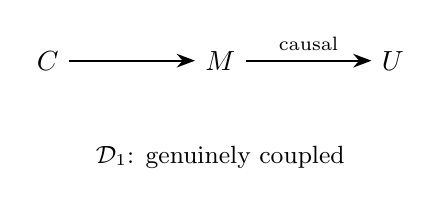
\begin{tikzpicture}[>=Stealth, thick, node distance=16mm]
  \node (C1) {$C$};
  \node[right=of C1] (M1) {$M$};
  \node[right=of M1] (U1) {$U$};
  \draw[->] (C1) -- (M1);
  \draw[->] (M1) -- (U1) node[midway, above, font=\scriptsize] {causal};
  \node[below=7mm of M1, font=\small] {$\mathcal{D}_1$: genuinely coupled};
\end{tikzpicture}
\hspace{18mm}
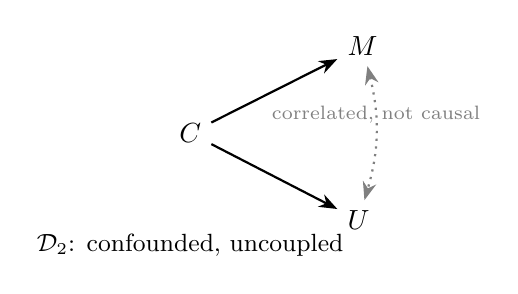
\begin{tikzpicture}[>=Stealth, thick, node distance=16mm]
  \node (C2) {$C$};
  \node[above right=6mm and 16mm of C2] (M2) {$M$};
  \node[below right=6mm and 16mm of C2] (U2) {$U$};
  \draw[->] (C2) -- (M2);
  \draw[->] (C2) -- (U2);
  \draw[gray, dotted, <->] (M2) to[bend left=15] node[midway, above, font=\scriptsize, gray] {correlated, not causal} (U2);
  \node[below=9mm of C2, font=\small] {$\mathcal{D}_2$: confounded, uncoupled};
\end{tikzpicture}
\caption{Both dyads induce the identical joint law over $(C,M,U)$ used in the proof of Theorem~\ref{thm:nonid}, so every observational functional $\Phi$ agrees on them. On the left, $M$ mediates the only path from $C$ to $U$: intervening on $M$ changes $U$. On the right, $U$ reads off $C$ directly; $M$ and $U$ are statistically associated (dotted) purely through their common cause, and intervening on $M$ leaves $U$ unchanged. $\mathcal{F}$ tracks the solid causal arrow into $U$, not the association.}
\label{fig:dags}
\end{figure}

\subsection{The result}

\begin{theorem}[Non-identifiability of functional coupling]\label{thm:nonid}
There exist dyads $\mathcal{D}_1$ and $\mathcal{D}_2$ such that
\[
P_1(Z_A, M, Z_B, U) \;=\; P_2(Z_A, M, Z_B, U) \qquad\text{yet}\qquad \mathcal{F}(\mathcal{D}_1) > 0 = \mathcal{F}(\mathcal{D}_2).
\]
Consequently no observational measure $\Phi$ identifies $\mathcal{F}$.
\end{theorem}

\begin{proof}
Let $C \sim \mathrm{Uniform}\{1,\dots,K\}$ with $K \geq 2$ denote a shared convention-bearing latent: the content the dyad has learned to coordinate on.

\emph{Dyad $\mathcal{D}_1$ (genuinely coupled).} The sender's state is $Z_A = C$; it emits $M = C$; the receiver's state is $Z_B = M$ and its behaviour is $U = M$. Here $B$ reads the channel and acts on what it reads.

\emph{Dyad $\mathcal{D}_2$ (confounded, uncoupled).} The sender's state is $Z_A = C$ and it emits $M = C$ exactly as before. The receiver, however, has independent access to $C$ through shared prior context, and sets $Z_B = C$, $U = C$, ignoring $M$ entirely.

Both dyads induce the same observational law: $Z_A = M = Z_B = U$ almost surely, uniform on $\{1,\dots,K\}$. Hence $P_1 = P_2$ and every functional of the observational distribution agrees on them. In particular $I(Z_A;Z_B) = I(M;U) = \log K$ in both --- both dyads look maximally coupled by every available measure, including measures defined on behaviour.

Now intervene. In $\mathcal{D}_1$, setting $\mathrm{do}(M = m')$ yields $U = m'$, so $P(U \mid \mathrm{do}(M{=}m))$ varies with $m$ and $\mathcal{F}(\mathcal{D}_1) = \log K > 0$. In $\mathcal{D}_2$, setting $\mathrm{do}(M = m')$ leaves $U = C$ unchanged, so $P(U \mid \mathrm{do}(M{=}m))$ is constant in $m$ and $\mathcal{F}(\mathcal{D}_2) = 0$.

Since $\Phi$ depends on the dyad only through $P$, and $P_1 = P_2$ while $\mathcal{F}_1 \neq \mathcal{F}_2$, no $\Phi$ can equal $\mathcal{F}$.
\end{proof}

\begin{remark}
The construction is elementary; that is the point. The mathematical content is standard confounding. The substantive claim is about \emph{where} it applies: not to a badly designed study that could be fixed, but to every dyad capable of communicating at all, because shared convention is a precondition rather than a nuisance. One cannot randomise away the common cause without destroying the phenomenon.
\end{remark}

\begin{remark}[The case that matters most]
$\mathcal{D}_2$ is not a contrived pathology. It is a compact description of a large language model in conversation with a person. The model was trained on the recorded output of human convention; the user is a member of the culture that produced it. Both parties therefore hold $C$ independently, and their exchanges cohere \emph{whether or not} the user's particular signal is doing causal work. Fluency is exactly what $\mathcal{D}_2$ predicts. This is why conversational impressions of understanding are not merely unreliable but uninformative in principle.
\end{remark}

\begin{corollary}[Invalidity of conversational evaluation]\label{cor:turing}
Any evaluation procedure that scores a system solely on the distribution of exchanged signals and responses --- the imitation game and its descendants, dialogue benchmarks, human preference ratings --- is a functional of $P$ and therefore fails to identify $\mathcal{F}$. Such procedures cannot distinguish $\mathcal{D}_1$ from $\mathcal{D}_2$ at any sample size.
\end{corollary}

\begin{corollary}[Optimisation is indifferent]\label{cor:rlhf}
Training that maximises an observational score $\Phi$ applies pressure that is by construction identical on $\mathcal{D}_1$ and $\mathcal{D}_2$. Feedback schemes that rate outputs therefore cannot select for functional coupling except through whatever correlation happens to hold in the training distribution. This is not a claim that current systems lack functional coupling; it is the claim that the training signal does not distinguish, so any such coupling is incidental to the objective rather than selected by it.
\end{corollary}

\section{When identification is possible}\label{sec:identification}

Theorem~\ref{thm:nonid} is a negative result about observational data absent further assumptions. It is not the claim that functional coupling can never be estimated. This section characterises what suffices --- and, more usefully for practice, what does not. The negative results in \S\ref{sec:insufficient} are the ones with consequences for existing literature.

\subsection{Sufficient conditions}

\begin{theorem}[Identification]\label{thm:id}
Functional coupling $\mathcal{F}(\mathcal{D})$ is identified if any of the following holds. Informally: you can see the confounder and adjust for it; you can find something that jitters the message for reasons unrelated to the convention and use it as leverage; or you can just set the message yourself.
\begin{enumerate}[label=(\roman*), leftmargin=*, itemsep=2pt]
    \item \textbf{Adjustment.} The convention-bearing latent $C$ is observed and satisfies the back-door criterion relative to $(M, U)$. Then
    $P\big(U \mid \mathrm{do}(M{=}m)\big) = \sum_c P(U \mid M{=}m, C{=}c)\,P(c)$.
    \item \textbf{Instrument.} There exists $N$ with $N \to M$, $N \perp\!\!\!\perp C$, and $N$ influencing $U$ only through $M$. Under standard auxiliary assumptions (linearity, or monotonicity in the discrete case) $\mathcal{F}$ is point-identified; absent them it is partially identified, with informative bounds.
    \item \textbf{Intervention.} The experimenter can set $M$ directly. Then $\mathcal{F}$ is identified by Definition~\ref{def:fc}.
\end{enumerate}
\end{theorem}

\begin{proof}
(i) is back-door adjustment and (ii) instrumental-variable identification, both standard \cite{pearl2009causality}; (iii) is immediate from the definition.
\end{proof}

\begin{remark}[On (i): rarely available]
Adjustment is the condition one would most like to have and least often does. Convention is precisely what is implicit, distributed, and unarticulated between two parties; a researcher able to write down $C$ in full has already solved a harder problem than the one at hand. Proxies exist --- measured familiarity or shared history for human dyads, overlap between a user's idiom and a model's training distribution for human--AI pairs --- but adjustment on a proxy yields partial control, not identification, and the residual confounding is of unknown sign.
\end{remark}

\begin{remark}[On (ii): an underexploited inversion]\label{rem:noise}
The instrumental route is the practically interesting one, because instruments in this setting are often already present and are currently discarded. \emph{Exogenous channel noise is an instrument.} Transmission dropout, trial-to-trial jitter, latency variability, hardware artefact --- any perturbation of the transmitted signal that is independent of the dyad's shared convention satisfies the requirements. This inverts the usual methodological posture: noise in the channel, ordinarily treated as a nuisance to be minimised or regressed away, is exactly what renders functional coupling estimable without intervening. Studies that carefully denoise their channel may be discarding their only source of identification.

We verify this constructively. In a linear-Gaussian pair of dyads matching Theorem~\ref{thm:nonid}'s construction --- $M = C + N$ with $N$ exogenous and independent of $C$, and $U$ set to depend causally on $M$ (coupled) or on $C$ directly with $M$ inert (confounded), calibrated so $\mathrm{Cov}(M,U)$ is identical across the two --- the naive observational regression of $U$ on $M$ is statistically indistinguishable between them ($0.800 \pm 0.005$ vs.\ $0.799 \pm 0.019$ across 200 seeds), while the instrumental estimate $\mathrm{Cov}(U,N)/\mathrm{Cov}(M,N)$ recovers $0.800 \pm 0.007$ for the coupled dyad and $-0.003 \pm 0.034$ for the confounded one, matching each dyad's true interventional effect exactly. This holds only once the instrument is strong enough: a first-stage $F$-statistic below $\sim$10 (weak exogenous variance) makes the IV estimate uninformative in either direction, so the diagnostic must be reported alongside the estimate, not assumed. Code and full sweep in \texttt{experiments/paper2\_identifiability/noise\_as\_instrument.py}.
\end{remark}

\subsection{What does not suffice}\label{sec:insufficient}

\begin{proposition}[Temporal precedence is insufficient]\label{prop:time}
Measures defined by temporal ordering do not identify $\mathcal{F}$. Because $C$ precedes both $M$ and $U$, conditioning on the past of $U$ does not block the back-door path $M \leftarrow Z_A \leftarrow C \rightarrow U$. Transfer entropy, Granger causality, and directed information therefore remain functionals of the observational distribution and fall under Theorem~\ref{thm:nonid}.
\end{proposition}

This deserves emphasis because such measures are routinely described as ``directed'' or ``causal,'' and the governing intuition is that respecting temporal order supplies causal content. It does so only in the absence of a common cause preceding both variables. In dyadic communication such a common cause is not a hazard to be checked for but a structural guarantee: without prior shared convention there is no communication to measure. The field's principal workhorse is thus subject to the theorem in full.

\begin{proposition}[Receiver-side measurement is insufficient]\label{prop:frontdoor}
Observing the receiver's internal state does not restore identification via the front-door criterion --- Pearl's route for identifying a causal effect through a mediator when the direct treatment--outcome relationship is itself confounded, which requires no back-door confounding between treatment and mediator and none between mediator and outcome (except what the treatment already blocks). Consider $Z_B$ as candidate mediator on $M \to Z_B \to U$. Front-door identification requires (a) no unblocked back-door path from $M$ to $Z_B$, and (b) that every back-door path from $Z_B$ to $U$ be blocked by $M$. If $C \to Z_B$ and $C \to U$, then $M \leftarrow Z_A \leftarrow C \rightarrow Z_B$ violates (a), and $Z_B \leftarrow C \rightarrow U$ --- which conditioning on $M$ does not block --- violates (b).
\end{proposition}

Both edges are present whenever the receiver's internal representations and its behavioural dispositions were shaped by the same prior convention, which is to say whenever the receiver is capable of communicating at all.

\begin{corollary}\label{cor:resolution}
Neither higher-resolution neural recording nor finer activation-level interpretability restores identification. Proposition~\ref{prop:frontdoor} concerns causal structure, not measurement precision, and is therefore invariant to improvements in either.
\end{corollary}

Corollary~\ref{cor:resolution} combines with the empirical result of the next section to give receiver-side measurement a double failure: it targets the wrong node, and it cannot be adjusted into targeting the right one.

\section{The state--behaviour gap}\label{sec:empirical}

Theorem~\ref{thm:nonid} concerns confounding. We now show a second, logically independent failure: even with no confounding and complete ground truth, coupling measured at the level of internal states does not imply functional coupling.

\begin{proposition}[State--behaviour gap]\label{prop:gap}
There exist dyads in which $I(M; Z_B)$ is near its maximum while $\mathcal{F} = 0$.
\end{proposition}

We establish this constructively, in a system where every variable is observable and the causal structure is known by construction.

\subsection{System}

Two neural-network agents were trained jointly in a referential navigation task (PettingZoo \texttt{simple\_speaker\_listener}, \cite{terry2021pettingzoo}). A \emph{speaker} observes a private goal --- which of three landmarks the partner must reach --- and cannot move. A \emph{listener} observes its own position and the landmarks but not the goal, and must navigate. The environment's fixed vocabulary was bypassed in favour of a learned discrete channel of tunable width, using a straight-through Gumbel--Sigmoid relaxation so that gradients flow from the listener's loss into the speaker's message \cite{jang2016categorical, foerster2016learning}. Agents were trained with policy gradients and an auxiliary reconstruction objective that pressures the message to carry the goal. Full configuration and code accompany this manuscript.

Three quantities were measured after training, on frozen policies:

\begin{itemize}[leftmargin=*, itemsep=1pt]
    \item \textbf{Encoding fidelity} --- $R^2$ of a regression predicting the emitted message from the speaker's private goal. This is a \emph{positive signalling} measure in the sense of \cite{lowe2019pitfalls}.
    \item \textbf{Representational uptake} --- reconstruction error of a decoder reading the goal from the listener's hidden layer, i.e.\ whether the goal is present and linearly available in the receiver's internal state. This is the artificial analogue of cross-subject decoding in neuroimaging and of feature discovery in interpretability.
    \item \textbf{Functional coupling} --- the behavioural consequence of the message, estimated by intervention, in the two forms of \S\ref{sec:remedy}. \emph{Ablation} replaces the message with zeros. \emph{Randomisation} replaces it with a real, in-distribution message the speaker genuinely emitted on a different episode, preserving the message marginal exactly while destroying the message--state pairing. Both are direct estimates of Definition~\ref{def:fc}; we report standardised effects $z$ against the intact condition.
\end{itemize}

\subsection{Result}

\begin{table}[h]
\centering
\small
\begin{tabular}{@{}p{0.50\textwidth} c p{0.25\textwidth}@{}}
\toprule
\textbf{Quantity} & \textbf{Measured} & \textbf{Interpretation} \\
\midrule
Encoding fidelity (speaker $\to$ message) & $R^2 = 0.90$ & message carries the goal \\
Representational uptake (message $\to$ receiver state) & recon.\ error $0.0017$ & goal present in receiver \\
Message sensitivity of policy (KL, real vs.\ shuffled) & $0.021$ nats & \\
Own-state sensitivity of policy (KL, reference scale) & $0.686$ nats & $\sim$33$\times$ larger \\
\midrule
Functional coupling --- \emph{ablation} (message zeroed) & $z = +0.50$ & no detectable effect \\
Functional coupling --- \emph{randomisation} (message mispaired) & $z = +1.82$ & small, marginal effect \\
\textbf{Share of available value of information captured} & $\mathbf{\lesssim 12\%}$ & \textbf{performance at goal-blind optimum} \\
\bottomrule
\end{tabular}
\caption{State-level coupling at ceiling; functional coupling small at best, and yielding no task benefit.}
\label{tab:gap}
\end{table}

The message demonstrably carries the goal. The goal is demonstrably present in the receiver's internal representation, recoverable by a linear readout at negligible error. Under ablation, behaviour is statistically indistinguishable from behaviour with the channel zeroed.

Randomisation, however, is not null: destroying the message--state pairing while preserving the message marginal costs $2.3$ reward units ($z = +1.82$), against $0.6$ units for outright ablation. Two conclusions follow, and the second matters more than the first.

\textbf{Randomisation is the more sensitive instrument.} It detects a residual behavioural dependence on message content that ablation misses --- roughly a threefold larger standardised effect on the same trained system. We had predicted this ordering on theoretical grounds in \S\ref{sec:remedy}; it is here confirmed empirically. A zeroed channel presents a constant, easily accommodated input, whereas a mispaired but in-distribution message actively misleads any receiver retaining sensitivity to content. Practitioners adopting the protocol of \S\ref{sec:remedy} should prefer randomisation, and should not read a null ablation result as establishing zero functional coupling.

\textbf{But the residual sensitivity does no work.} The relevant scale is the value of the information itself. In this environment an analytic policy that uses the goal scores $-8.78$ and the best goal-blind policy scores $-16.88$ (Table~\ref{tab:oracle}), so knowing the goal is worth $8.10$ reward units. The trained receiver scores $-15.87$: statistically at the goal-blind optimum, capturing at most $\sim$$12\%$ of the available value, and that residual is itself marginal. So the receiver's behaviour is faintly perturbable by the message while extracting essentially none of its value.

This is a sharper statement of the dissociation than a flat null would have been. \emph{Behavioural sensitivity and functional benefit are themselves distinct.} A receiver can be measurably influenced by a signal and still derive no advantage from it --- which means that even an interventional measure must be calibrated against what the information is worth, not merely tested against zero. We accordingly report the captured share of the value of information as the primary quantity, and recommend it over a bare significance test.

\subsection{The infinite-bandwidth control}

A natural objection is that some residual channel imperfection is responsible. We removed the channel.

In a separate condition the listener was given the speaker's private goal \emph{directly}, concatenated to its own observation --- no encoder, no bottleneck, no discretisation, no noise. This is the limiting case of a perfect interface.

\begin{table}[h]
\centering
\small
\begin{tabular}{lc}
\toprule
\textbf{Policy} & \textbf{Return} \\
\midrule
Analytic expert (uses the goal optimally) & $-8.78 \pm 7.76$ \\
Goal-blind heuristic (hedges to landmark centroid) & $-16.88 \pm 9.84$ \\
Random & $-41.94 \pm 34.84$ \\
\midrule
Trained agent, learned channel & $\approx -16$ \\
\textbf{Trained agent, direct goal access (no channel)} & $\mathbf{-15.96 \pm 9.70}$ \\
\bottomrule
\end{tabular}
\caption{An agent handed the goal for free converges to the goal-blind optimum.}
\label{tab:oracle}
\end{table}

The agent with free, perfect, noiseless access to the information converged to $-15.96$: the score of the goal-blind heuristic, and indistinguishable from agents that received nothing. An analytic policy that uses the goal achieves roughly twice the return, so the information was both available and valuable. It was not used, and further training did not change this.

This is the strongest form of the dissociation. The failure is not attributable to bandwidth, noise, encoding, alignment, or capacity, because in this condition none of those exist.

\begin{remark}[A methodological aside]
During this work an earlier analysis reported a clean monotone relationship between channel bandwidth and measured transfer entropy ($r = 0.99$), apparently confirming a capacity law. It was an artefact: the estimator is an in-sample regression whose bias grows with the ratio of channel dimension to sample size, and a pure-noise control returned $0.71$ ``bits'' of coupling where the true value was zero. Applying a block-shuffled surrogate correction removed essentially the entire effect. We report this because it illustrates the paper's thesis at the level of practice: observational coupling measures can produce confident, well-behaved, theoretically congenial numbers in the complete absence of coupling.
\end{remark}

\section{Why the gap exists}\label{sec:why}

The dissociation is not an artefact of weak optimisation, and understanding why illuminates the general case.

Coupling is not a property of a channel. It is a jointly held convention, and conventions are attractors of a shared history rather than consequences of contact. Two facts follow.

\textbf{Coupling cannot be established unilaterally.} Information has value to a system only if that system already possesses machinery that acts on it; acquiring that machinery is rewarded only if the information is already being acted upon. Each half is a precondition for the other, so neither party can move first. Meanwhile there is always a policy available that ignores the partner and performs moderately well alone --- in our system, hedging toward the centroid of the candidate landmarks. That policy is reachable immediately, unilaterally, without coordination. It is found early and it is stable: viewed from inside it, the partner's signal is worth nothing, so no local gradient points out of it.

Our agents fell into precisely this attractor and never left, with the answer sitting in their own hidden layer the entire time. We tested four independent escapes --- exploration pressure, gradient batching, an information-aware value baseline, and an auxiliary objective on the receiver --- and none produced behavioural change, because each optimises \emph{within} the basin rather than across its boundary.

\textbf{Coupling should therefore be bistable, and hence historical.} If coupling is an attractor rather than a channel state, the conditions under which it ignites need not match the conditions under which an established convention collapses. We predict hysteresis: a dyad that has already established a convention will sustain coupling under degradation that would have prevented its formation. If this holds, coupling capacity is not a function of a dyad's present parameters at all, only of its history --- and cross-sectional measurement of coupling capacity is ill-posed. This also explains an everyday asymmetry: establishing a shared code, whether a language, a jargon, or a couple's private shorthand, is enormously expensive, while maintaining one is nearly free.

\section{The remedy: interventional coupling measurement}\label{sec:remedy}

The diagnosis prescribes the treatment. Functional coupling is defined interventionally, is not identified observationally, and must therefore be estimated by intervention.

\begin{quote}
\textbf{Protocol.} To establish that a signal is doing work, ablate or randomise it and measure the change in the receiver's behaviour. Functional coupling is what survives removal of the signal.
\end{quote}

Three practical forms, in increasing order of strength:

\begin{enumerate}[leftmargin=*, itemsep=2pt]
    \item \textbf{Ablation.} Replace the signal with a null or constant and measure the behavioural difference. Establishes whether the channel carries any functional load.
    \item \textbf{Randomisation.} Replace the signal with one drawn from the same marginal but paired with a different underlying state. This is the decisive test against the confound of Theorem~\ref{thm:nonid}: it preserves every surface property of the signal while destroying its relationship to the sender's state. A receiver acting on shared prior convention rather than on the message is unaffected; a genuinely coupled receiver degrades.
    \item \textbf{Targeted perturbation.} Alter the signal so as to change its meaning under the putative convention while holding surface statistics fixed, and check that behaviour tracks the altered meaning. Establishes not only that the channel matters but that it matters \emph{in the way the convention specifies}.
\end{enumerate}

Randomisation deserves emphasis: it is what defeats $\mathcal{D}_2$. Under $\mathrm{do}(M = m')$ with $m'$ drawn independently of $C$, the coupled dyad's behaviour changes and the confounded dyad's does not, which is exactly the discrimination Theorem~\ref{thm:nonid} shows observation cannot make. Section~\ref{sec:empirical} confirms empirically that it is also the more sensitive of the two, detecting residual dependence that ablation reports as null.

A final and easily missed point: an interventional test still requires a \emph{scale}. Establishing that behaviour changes when a signal is removed does not establish that the signal is doing appreciable work. We recommend reporting the effect as a fraction of the value of the information --- the return difference between an optimally informed and an optimally uninformed policy --- since that quantity is what a claim of functional coupling should be measured against. Where the informed optimum is unavailable, the uninformed optimum alone still provides a far more meaningful reference than zero.

\section{Implications}\label{sec:implications}

\subsection{Evaluation of AI systems}
By Corollary~\ref{cor:turing}, conversational and preference-based evaluation cannot identify functional coupling between a model and a user's intent. This is a structural limitation, not a matter of benchmark quality or rater training. The prescription is concrete: evaluate by intervention. Perturb the user's signal in ways that change intent while preserving surface form, and measure whether model behaviour tracks the change. A system whose outputs are invariant to such perturbations is exhibiting $\mathcal{D}_2$ --- coherent, fluent, and uncoupled.

We note the practical stake. Apparent and functional coupling produce identical behaviour \emph{within} the distribution on which apparent coupling was established, and divergent behaviour outside it. Our receiver looked unremarkable --- it scored what every other agent scored --- until the situation actually required the signal, at which point it failed completely. On this account a familiar deployment pattern, in which systems pass extensive evaluation and then fail in the field, is not a symptom of insufficient testing but of testing a quantity that does not determine the one that matters.

\subsection{Mechanistic interpretability}
A claim that a model represents some quantity is a statement about decodability from internal state --- precisely the measure that read $0.0017$ in Table~\ref{tab:gap} while behaviour read zero. Presence of a feature in a representation licenses nothing about its causal role. The field's causal methods --- activation patching, causal scrubbing, and related interventions \cite{geiger2021causal} --- are therefore not refinements of decoding-based analysis but the only valid form of the claim. Our result is a clean existence proof of a feature that is fully present, linearly recoverable, and behaviourally inert.

Corollary~\ref{cor:resolution} sharpens this into a claim about the field's trajectory. Because the obstruction is structural, it is not relieved by better probes, larger probing datasets, or finer-grained feature decomposition: a decoding result of arbitrarily high fidelity still licenses no behavioural conclusion. Progress on decoding accuracy and progress on causal warrant are therefore orthogonal, and effort spent on the former should not be scored as progress on the latter.

\subsection{Hyperscanning and inter-brain coupling}
Inter-brain synchrony and directed-information measures are observational, state-level, and applied to dyads that share both a task and a culture --- that is, a large common cause. Three of our results bear on this simultaneously, and their conjunction is unusually restrictive. Theorem~\ref{thm:nonid} applies directly. Proposition~\ref{prop:time} closes the most natural escape: transfer entropy and Granger causality are the field's standard instruments precisely because they are directional, but directionality obtained from temporal ordering does not survive a common cause that precedes both series, and shared convention is exactly such a cause. Proposition~\ref{prop:frontdoor} closes the second: recording more of the receiving brain, at higher resolution, does not help, because the failure is structural rather than one of measurement precision. And Proposition~\ref{prop:gap} adds that even were confounding absent, the quantity being measured is at the wrong node. Reported inter-brain coupling therefore establishes that two brains' states covary; it does not establish that either brain's behaviour depends on the other's signal.

There is, however, a constructive path that does not require new experiments. By Remark~\ref{rem:noise}, exogenous variability in the transmitted signal --- momentary occlusion, acoustic interference, dropped words, latency --- is an instrument, provided it is independent of the pair's shared history. Existing hyperscanning corpora contain such variation and typically treat it as noise to be cleaned. Recovering it and using it as an instrument is, to our knowledge, an unexploited route to interventional conclusions from already-collected observational data. We suggest that inter-brain studies adopt signal randomisation as a standard control, and note a testable consequence: on a fixed task with fixed instrumentation, measured coupling should track the pair's \emph{prior shared convention} --- strangers below acquaintances below long-term partners --- and that effect should exceed any channel-quality variable.

\subsection{Brain-to-brain interfaces}\label{sec:bbi}
The framework retrodicts a standing anomaly, and the anomaly is documented rather than asserted. Rao et al.\ \cite{rao2014direct} (2014, 64-channel EEG sender, one TMS coil, three pairs) transmitted $0.25$--$0.81$ bits/trial. Jiang et al.\ \cite{jiang2019brainnet} (2019, BrainNet: a real-time, three-person, two-sender architecture, the field's most technically advanced system) transmitted $0.336$ bits/trial for its best sender --- \emph{less} than Rao's best pair five years earlier, despite strictly more sophisticated hardware and only a single electrode (Oz) actually used for decoding out of the 8-- and 32-channel systems available. The authors state this themselves: ``From the first human BBI to BrainNet, the level of information complexity has remained binary\ldots [and] this low bit rate required a disproportionate amount of technical hardware and setup'' \cite{jiang2019brainnet}. An independent systematic review of the 2013--2020 literature \cite{nam2021prisma} reports the same pattern across the full set of published studies: methodological diversification (EEG, intracortical microelectrodes, focused ultrasound, optogenetics; TMS, direct cortical stimulation) without a corresponding rise in bits transmitted, concluding that mutual information ``has been limited to mostly binary information transfer'' throughout. On a channel-centric account this is unexplained, and worsens with better hardware rather than improving. On the present account it is forced: in every such study the convention is installed from outside, in advance, by ordinary language --- the participant is \emph{told} that a phosphene means ``rotate,'' or the meaning is fixed by the experimenter's choice of stimulation site. Throughput is therefore bounded not by hardware but by how much convention can be pre-installed by talking to a subject beforehand. That bound is low and does not move when the hardware improves; if anything, coordinating a second sender in BrainNet added convention-installation overhead without adding transmitted content. Full study-by-study tabulation and sourcing in \texttt{literature/bbi\_throughput\_survey.md}.

\section{Related work}\label{sec:related}

The components of this argument exist; the synthesis and the identifiability claim, to our knowledge, do not.

Shannon explicitly excluded semantics from the engineering problem \cite{shannon1948mathematical}, a simplification that was safe while receivers executed protocols fixed in advance and fails once both ends must acquire their protocol. Pearl's causal hierarchy \cite{pearl2009causality} supplies the ladder on which we locate functional coupling. Searle's Chinese Room \cite{searle1980minds} argued that syntactic competence does not constitute understanding but offered no test; our contribution can be read as supplying an operational criterion and explaining why conversational tests could never have provided one.

Lewis formalised convention \cite{lewis1969convention}; Harnad posed symbol grounding \cite{harnad1990symbol}; Skyrms derived meaning from signalling games \cite{skyrms2010signals}. Kolchinsky and Wolpert \cite{kolchinsky2018semantic} give the nearest formal neighbour, defining semantic information as information with causal relevance to a system's viability --- like us, they locate meaning in causal consequence rather than correlation; unlike us, they do not address identifiability from observational data or the constitutive role of shared convention as confounder, and their formalism is monadic --- one system's information about its environment --- rather than dyadic, which is the structural reason it does not already reach the coupling question we ask.

In emergent communication, Lowe et al.\ \cite{lowe2019pitfalls} distinguish positive signalling from positive listening and warn that the former can be high while the latter is absent --- a distinction we rediscovered empirically before encountering their terminology, and which Table~\ref{tab:gap} instantiates with ground truth. Their matrix-communication-game experiments give an independent replication in a different environment: positive signalling (their Speaker Consistency, 0.19--0.54 across game sizes) coexists with causal influence at the floor, message removal leaving action-prediction accuracy essentially unchanged. They trace this to an architectural confound --- shared hidden layers between action and communication heads induce spurious signalling correlations even with untrained communication parameters. Our diagnostic chain rules out that mechanism for our system (separate networks, an auxiliary loss that raises encoding fidelity to $R^2=0.90$, and a listener reconstruction head that decodes the goal at error $0.0016$) and the dissociation persists regardless --- the same symptom, via a different route, which is why we read their result as a second instance of the phenomenon rather than an explanation of ours. They frame the finding as a metric pitfall with a practical remedy (measure causal influence, use several estimators); we argue no estimator escapes it without intervention. Eccles et al.\ \cite{eccles2019biases} introduce explicit biases to induce both, motivated by the joint-exploration failure our Section~\ref{sec:why} describes; Foerster et al.\ \cite{foerster2016learning} address the same obstacle architecturally. In AI safety, eliciting latent knowledge poses a closely related problem of separating what a system reports from what it uses. Interpretability's causal turn \cite{geiger2021causal} already reflects awareness that decoding is insufficient; we supply an argument for why intervention is necessary rather than merely preferable.

\section{Limitations and falsification}\label{sec:limits}

We state the ways this could be wrong, in order of severity.

\textbf{The assumption set may be narrowable further.} Theorem~\ref{thm:id} gives three sufficient conditions and Propositions~\ref{prop:time}--\ref{prop:frontdoor} rule out two tempting shortcuts, but we do not claim this characterisation is exhaustive. A weaker assumption set that still identifies $\mathcal{F}$ --- particularly one satisfiable in observational hyperscanning corpora, where intervention is impossible after the fact --- would be a substantial improvement and is where we would look first to strengthen the paper. Relatedly, our instrumental route (Remark~\ref{rem:noise}) is now demonstrated on a linear-Gaussian toy matching Theorem~\ref{thm:nonid}'s construction, but not yet on a system we did not design to make it work --- the natural next step is the existing Stage~2 RL testbed or a real hyperscanning corpus's channel dropout, where linearity and the noise's independence from shared history are no longer guaranteed by construction.

\textbf{The empirical demonstration is a single system.} Proposition~\ref{prop:gap} is an existence proof, which is what it needs to be, but it does not establish that the gap is common in systems of practical interest. If ablation and observational measures agree across a broad range of real dyads, the correction we prescribe is unnecessary in practice even if valid in principle.

\textbf{Functional coupling here is small, not provably zero.} The randomisation effect ($z = +1.82$) is marginal by conventional standards and we do not claim it is null; a larger evaluation set would sharpen it in one direction or the other. Our claim is the weaker and better-supported one that the receiver captures almost none of the available value of the information while every state-level measure is at ceiling. Readers should note that this makes the dissociation a matter of degree, and that our recommended statistic --- captured share of the value of information --- is what carries the argument, not a significance test.

\textbf{Hysteresis is predicted, not shown.} Section~\ref{sec:why}'s bistability claim is untested. Coincident onset and collapse thresholds would falsify it and restore coupling to the status of a state variable of the connection.

\textbf{The retrodiction rests on few data points.} Section~\ref{sec:bbi} now cites measured bits/trial from the two best-documented studies (Rao 2014, Jiang 2019, five years apart, throughput flat-to-declining despite more sophisticated hardware) plus an independent systematic review's qualitative agreement, rather than asserting the pattern from memory. But it is still only two quantified anchor points bracketing a decade, not a dense time series, and a general web search for 2021--2026 human-to-human BBI work found no further quantified study either confirming or breaking the pattern --- an absence of evidence, not evidence of the pattern's continuation. A more exhaustive database search, or a new BBI study reporting a materially higher bit rate, would each bear directly on this claim.

\textbf{Scope.} We address functional coupling as defined in Definition~\ref{def:fc} and make no claim about phenomenal understanding, consciousness, or meaning in a richer sense. A reader who holds that understanding is not exhausted by causal influence on behaviour should read our results as necessary but not sufficient conditions.

\section{Conclusion}

Four fields ask whether one system understands another, and all four answer by observing the exchange. We have argued that this cannot succeed. Shared convention is the precondition of communication and simultaneously a common cause of what is sent and how the receiver acts, so genuinely coupled and merely coherent dyads can be observationally identical; and independently of that confound, a receiver's internal state can contain a signal in full while its behaviour ignores it entirely. We demonstrated the latter in a system where the sender encoded at $R^2 = 0.90$, the receiver's hidden layer carried the content to a reconstruction error of $0.0017$, and the receiver nonetheless performed at the goal-blind optimum, capturing at most a tenth of what the information was worth --- and where handing it that information directly, with infinite bandwidth and no noise, changed nothing at all. Along the way we found that the receiver's behaviour was faintly perturbable by the signal while deriving no advantage from it, so that sensitivity and benefit dissociate in their turn, and an interventional test needs a scale rather than a null.

Functional coupling is an interventional quantity. It has been measured observationally. That, rather than any deep obscurity in the phenomenon, is why the question of whether one mind understands another has resisted answer: the instrument was on the wrong rung. The remedy is available and cheap. Remove the signal, and see what changes.

\bibliographystyle{plain}
\bibliography{references}

\end{document}
